% +------------------------------------------------------------------------+
% | Reference manual page: Halffacet.tex
% +------------------------------------------------------------------------+
% | 14.05.2004   Peter Hachenberger
% | Package: Nef_3
% | 
\RCSdef{\RCSFacetRev}{$Revision$}
\RCSdefDate{\RCSFacetDate}{$Date$}
% +------------------------------------------------------------------------+

\ccRefPageBegin

%%RefPage: end of header, begin of main body
% +------------------------------------------------------------------------+


\begin{ccRefClass}[Nef_polyhedron_3<Traits>::]{Halffacet}

\ccDefinition

A halffacet is an oriented, rectilinear bounded part of a plane. The following
figure depicts the incidences to halfedges, vertices and the notion of facet
cycles.

\begin{ccTexOnly}
    \begin{figure}[bht]
        \begin{center}
          \parbox{0.4\textwidth}{%
              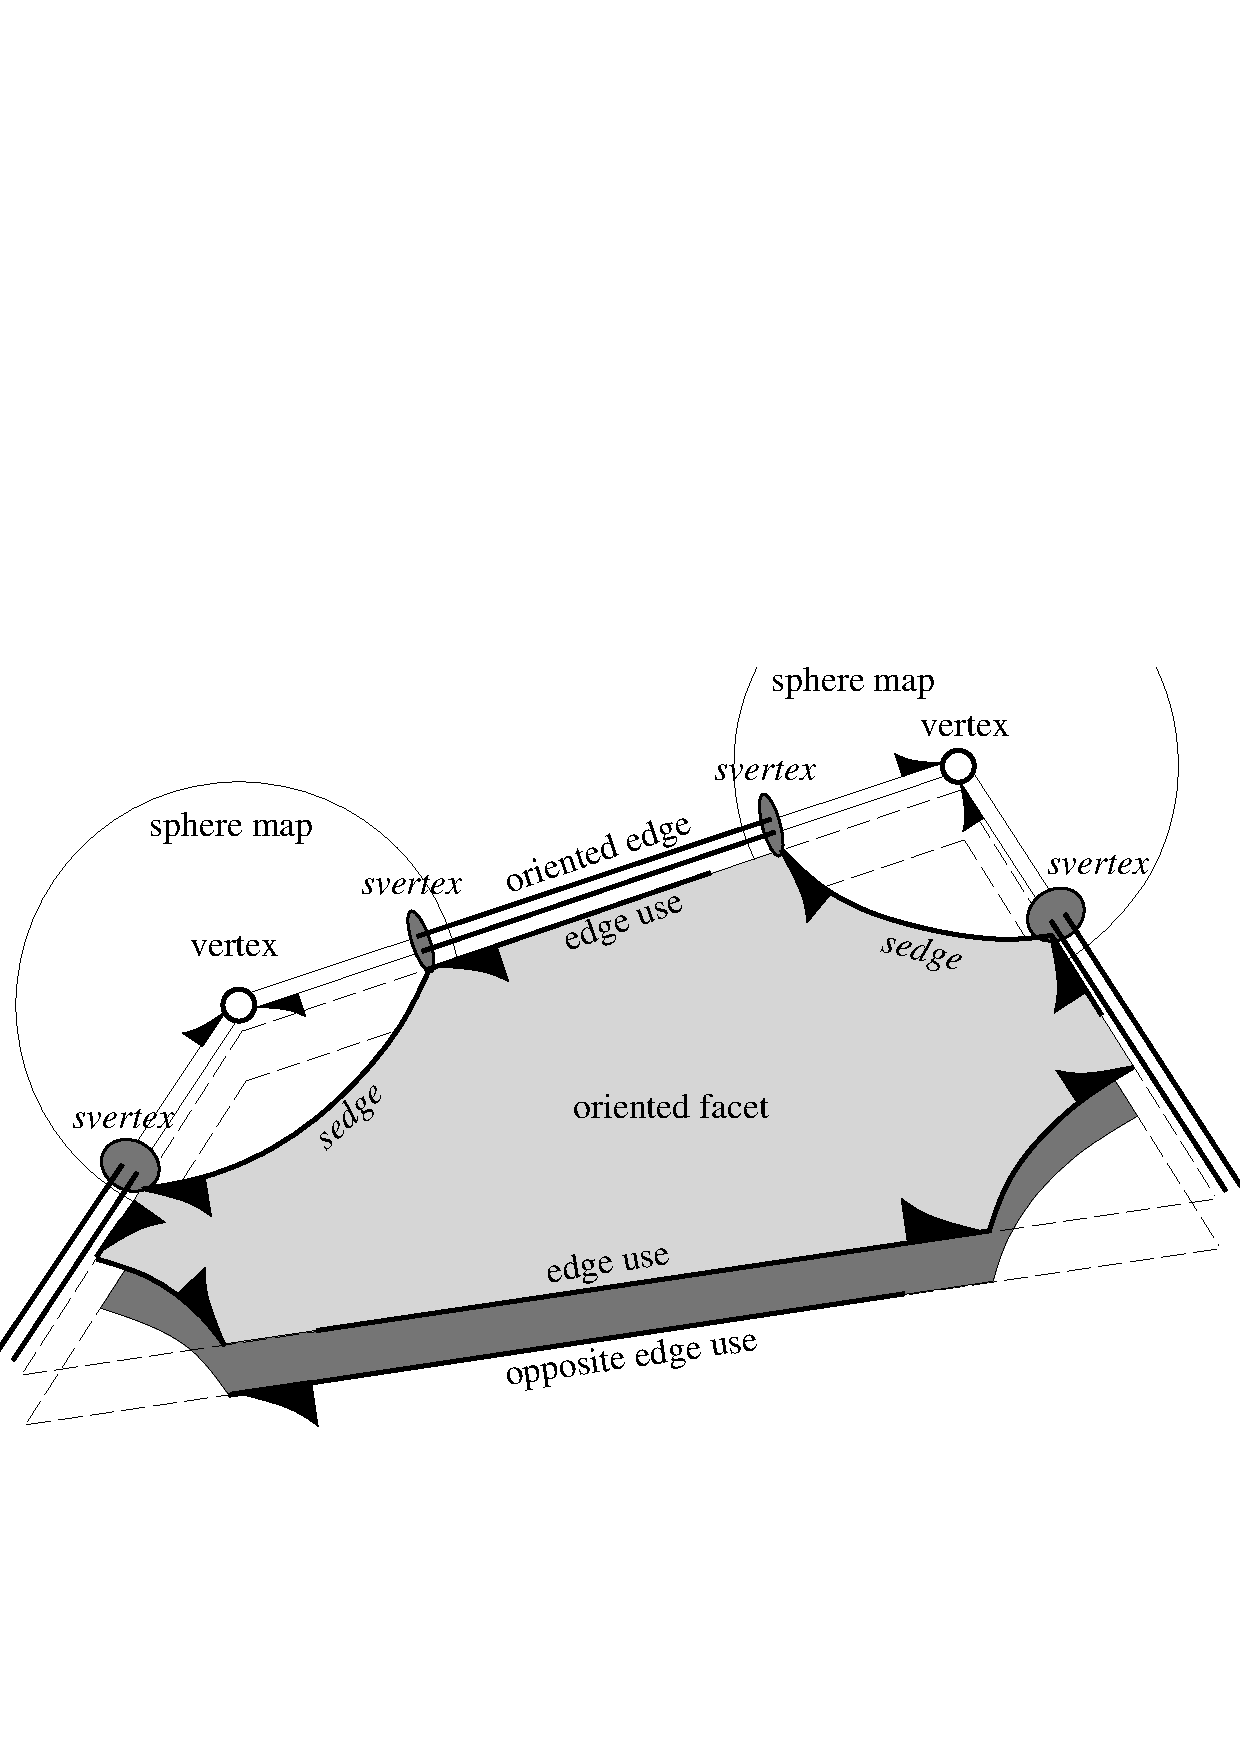
\includegraphics[width=0.4\textwidth]{Nef_3_ref/fig/snc}%
          }
        \end{center}
        \label{figureNef3FacetIncidences}
    \end{figure}
\end{ccTexOnly}

\begin{ccHtmlOnly}
    <CENTER>
    <A NAME="figureNef3HalffacetIncidences">
    <A HREF="fig/snc.gif">
        <img src="fig/snc.gif" 
             alt="Incidences of an Halffacet"></A><BR>
    <A HREF="fig/snc.gif">Figure:</A>
    </CENTER>
\end{ccHtmlOnly}

The member function \ccc{twin} returns the opposite halffacet, \ccc{incident_volume}
returns the incident volume. A Halffacet cycle either consists of consecutive
shalfedges along the border (or a hole) of the halffacet, or of a single
shalfloop on the sphere map of a vertex isolated on the halffacet. The 
iterator range (\ccc{halffacet_cycles_begin()}/\ccc{halffacet_cycles_end()})
provides an entry element for each halffacet cycle of a halffacet.

\ccInclude{CGAL/Nef_polyhedron_3.h}

\ccTypes
\ccThree{Halffacet_const_handle}{facet_cycles_begin();;}{}
\ccThreeToTwo

The following types are the same as in \ccc{Nef_polyhedron_3<Traits>}.

\ccNestedType{Mark}{type of mark.}

\ccNestedType{Plane_3}{plane type stored in Halffacet.}

\ccNestedType{Object_list}{list of Object handles.}

\ccNestedType{Halffacet_const_handle}{const handle to Halffacet.}
\ccGlue
\ccNestedType{Volume_const_handle}{const handle to volume.}
\ccGlue
\ccNestedType{Halffacet_cycle_const_iterator}
{const iterator over the entries to all halffacet cycles of a halffacet.}

\ccCreation
\ccCreationVariable{f}

There is no need for a user to create a \ccc{Halffacet} explicitly. The
class \ccc{Nef_polyhedron_3<Traits>} manages the needed halffacets internally.

%\ccConstructor{Halffacet();}{default constructor.}

%\ccConstructor{Halffacet(const Plane_3& h, Mark m);}
%{creates Halffacet with initial values for its mark and supporting plane.}

\ccThree{Halffacet_cycle_const_iterator}{facet_cycles_begin();;}{}

\ccOperations

\ccThree{Halffacet_cycle_const_iterator}{facet_cycle_begin();}{}

\ccMethod{const Mark& mark() const;}{the mark of \ccVar\ .}

\ccMethod{const Plane_3& plane() const;}{the supporting plane of \ccVar\ .}

\ccMethod{Halffacet_const_handle  twin() const;}{the twin of \ccVar\ .}

\ccMethod{Volume_const_handle  incident_volume() const;}{the incident volume of \ccVar\ .}

\ccMethod{Halffacet_cycle_const_iterator  facet_cycle_begin() const;}
{iterator over the entries to all halffacet cycles of \ccVar\ .}

\ccMethod{Halffacet_cycle_const_iterator  facet_cycle_end() const;}
{past-the-end iterator.}

\ccSeeAlso

\ccRefIdfierPage{CGAL::Nef_polyhedron_3<Traits>::Volume}\\
\ccRefIdfierPage{CGAL::Nef_polyhedron_3<Traits>::Halfedge}\\
\ccRefIdfierPage{CGAL::Nef_polyhedron_3<Traits>::SHalfedge}


\ccTagDefaults
\end{ccRefClass}

% +------------------------------------------------------------------------+
%%RefPage: end of main body, begin of footer
\ccRefPageEnd
% EOF
% +------------------------------------------------------------------------+
